\begin{figure*}[t]
    \centering
    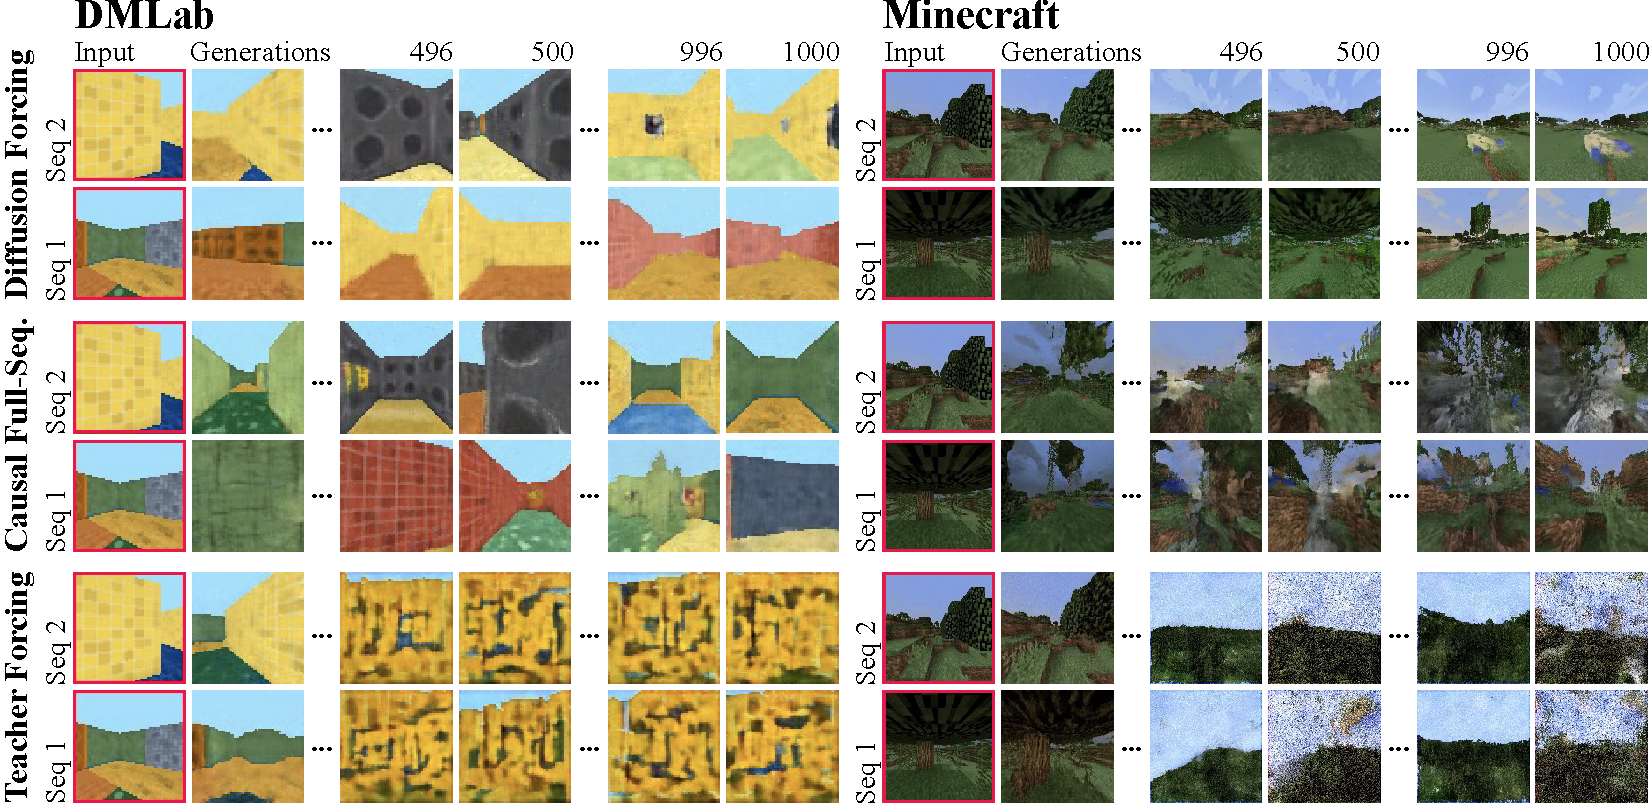
\includegraphics[width=\linewidth]{figures/pdf/Video_prediction.pdf}
    \caption{\textbf{Video Generation.} Among tested methods, \algons{} generations are uniquely temporally consistent and do not diverge even when rolling out well past the training horizon. Please see the \href{https://boyuan.space/diffusion-forcing}{\textcolor{blue}{project website}} for video results.}
    \label{fig:video_pred}
    \vspace{-5pt}
\end{figure*}

\section{Experiments}
We extensively evaluate \algons's merits as a generative sequence model across diverse applications in video and time series prediction, planning, and imitation learning. Please find the dataset and reproducibility details in the Appendix, as well as video results on the \href{https://boyuan.space/diffusion-forcing}{\textcolor{blue}{project website}}.



\subsection{Video Prediction: Consistent, Stable Sequence Generation and Infinite Rollout.}
\label{exp:video}
We train a convolutional RNN implementation of \algoseq{} for video generative modeling on videos of Minecraft gameplay~\cite{yan2023temporally} and DMLab navigation~\cite{yan2023temporally}. At sampling time, we perform auto-regressive rollout with stabilization proposed in Sec.~\ref{par:stabilizing_autoreg}.
We consider two baselines, both leveraging the same exact RNN architecture: a next-frame diffusion baseline trained with teacher forcing~\cite{teacher_forcing} as well as a causal full-sequence diffusion model. \cref{fig:video_pred} displays qualitative results of roll-outs generated by \algo{} and baselines starting from unseen frames for both datasets. While \algons{} succeeds at stably rolling out even far beyond its training horizon (e.g. $1000$ frames), teacher forcing and full-sequence diffusion baselines diverge quickly. Further, within the training horizon, we observe that full-sequence diffusion suffers from frame-to-frame discontinuity where video sequences jump dramatically, while \algo{} roll-outs show ego-motion through a consistent 3D environment. This highlights the ability of \algo{} to stabilize rollouts of high-dimensional sequences without compounding errors.



\begin{table*}[t]
\begin{picture}(\linewidth, 0.625\linewidth)
\put(0, 98){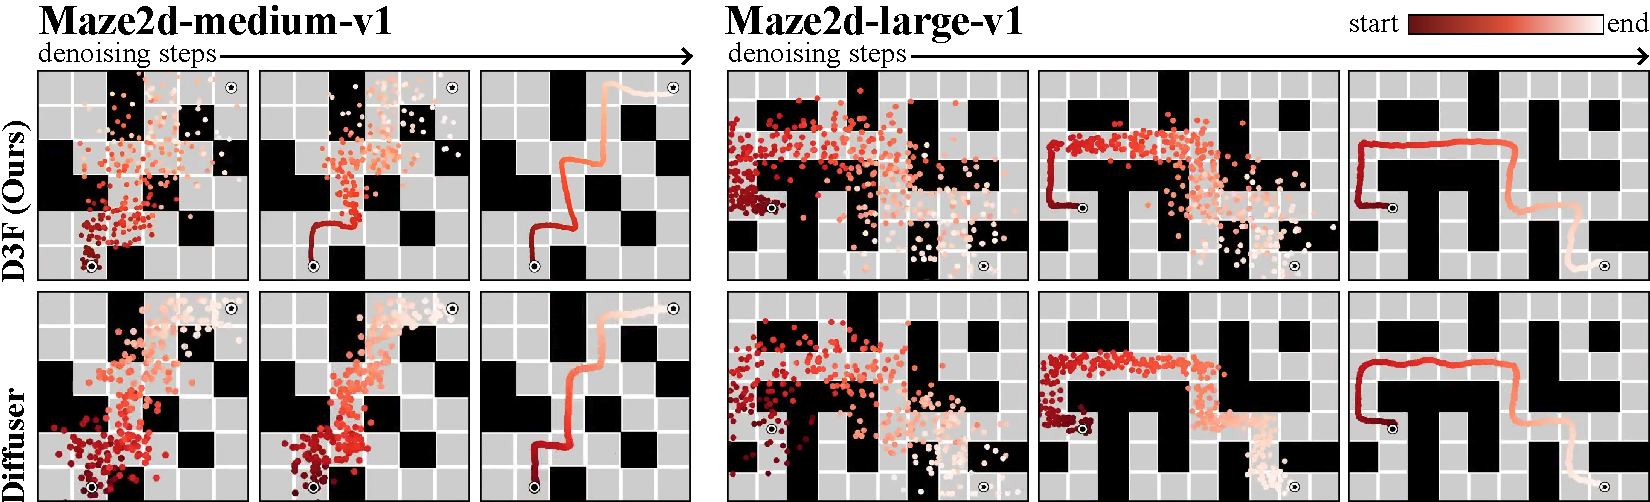
\includegraphics[width=\linewidth]{figures/pdf/Maze.pdf} }
\put(0, 43){
\resizebox{\linewidth}{!}{%
\begin{tabular}{@{}llccccccc@{}}
    \FL
    \multicolumn{2}{c}{\textbf{Environment}} & \textbf{MPPI} & \textbf{CQL} & \textbf{IQL} & \textbf{Diffuser*} & \textbf{Diffuser w/ diffused action} & \textbf{Ours wo/ MCG} & \textbf{Ours}\ML
    Maze2D & U-Maze & 33.2 & 5.7 & 47.4 & 113.9 \(\pm\) 3.1 & 6.3 \(\pm\) 2.1& 110.1 \(\pm\) 3.9 & \textbf{116.7 \(\pm\) 2.0} \NN
    Maze2D & Medium & 10.2 & 5.0 & 34.9 & 121.5 \(\pm\) 2.7 & 13.5\(\pm\)2.3 & 136.1 \(\pm\) 10.2 & \textbf{149.4 \(\pm\) 7.5} \NN
    Maze2D & Large & 5.1 & 12.5 & 58.6 & 123.0 \(\pm\) 6.4 & 6.3 \(\pm\)2.1 & 142.8 \(\pm\) 5.6 & \textbf{159.0 \(\pm\) 2.7} \ML
    \multicolumn{2}{c}{\textbf{Single-task Average}} & 16.2 & 7.7 & 47.0 & 119.5 & 8.7 & 129.67 & \textbf{141.7}  \ML[0.11em]
    Multi2D & U-Maze & 41.2 & - & 24.8 & 128.9 \(\pm\) 1.8 & 32.8\(\pm\)1.7 & 107.7 \(\pm\) 4.9 & \textbf{119.1 \(\pm\) 4.0} \NN
    Multi2D & Medium & 15.4 & - & 12.1 & 127.2 \(\pm\) 3.4 & 22.0\(\pm\)2.7 & 145.6 \(\pm\) 6.5 & \textbf{152.3 \(\pm\) 9.9} \NN
    Multi2D & Large & 8.0 & - & 13.9 & 132.1 \(\pm\) 5.8 & 6.9 \(\pm\)1.7 & 129.8 \(\pm\) 1.5 & \textbf{167.1 \(\pm\)2.7}  \ML
    \multicolumn{2}{c}{\textbf{Multi-task Average}} & 21.5 & - & 16.9 & 129.4 & 20.6 &  127.7 & \textbf{146.2} \LL
\end{tabular}
}
}
\end{picture}

\caption{ \textbf{\algons{} for Planning.} (\textbf{top}) During sampling, \algo{} allows each time step to be denoised on different noise schedules, enabling us to account for causal uncertainty during guided planning. \algo{} keeps the far future more uncertain than the near future while Diffuser~\cite{janner2022planning} puts them at the same noise level during sampling. (\textbf{bottom)} Quantitatively, \algo{} achieves the highest average reward across runs. Diffuser fails dramatically when executing the actually generated actions, requiring a hand-crafted PD controller (indicated by the asterisk) and ignoring generated actions.}
\vspace{-10pt}
\label{fig:planning}
\end{table*}



\subsection{Diffusion Planning: MCG, Causal Uncertainty, Flexible Horizon Control.}
\label{sec:exp_decision_making}
Decision-making uniquely benefits from \algo{}'s capabilities. We evaluate our proposed decision-making framework in a standard offline RL benchmark, D4RL~\cite{d4rl}. Specifically, we benchmark \algo{} on a set of 2D maze environments with sparse reward. An agent is tasked with reaching a designated goal position starting from a random starting position. In Appendix~\ref{app:dataset_detail} we provide a detailed description of the environment. The benchmark provides a dataset of \emph{random walks} through mazes (thus stochastic). We train one model per maze. 

We benchmark the proposed decision-making framework~\ref{sec:method_decision_making} with state-of-the-art offline RL methods and the recently introduced Diffuser~\cite{janner2022planning}, a diffusion planning framework. See Fig.~\ref{fig:planning} for qualitative and quantitative results: \algshort{} outperforms Diffuser and all baselines across all $6$ environments. 

\paragraph{Benefit of Monte Carlo Guidance.}
The typical goal for an RL problem is to find actions that maximize the \emph{expected} future rewards, which we achieve through MCG. Full-sequence diffusion models such as Diffuser do not support sampling to maximize expected reward, as we formally derive in \Cref{app:cannot_mcg}. To understand MCG's importance, we ablate it in \Cref{fig:planning}. Removing MCG guidance degrades our performance, though \algons{} remains competitive even then.

\paragraph{Benefit of Modeling Causality.}
Unlike pure generative modeling, sequential decision-making takes actions and receives feedback. Due to compounding uncertainty, the immediate next actions are more important than those in the far future.
Though Diffuser and subsequent models are trained to generate sequences of action-reward-state tuples $[\ba_t, \br_t, \bo_t]$, directly executing the actions will lead to a trajectory that deviates significantly from the generated states. In other words, the generated states and actions are not causally consistent with each other. To address this shortcoming, Diffuser's implementation ignores the generated actions and instead relies on a hand-crafted PD controller to infer actions from generated states. In Table~\ref{fig:planning}, we see that Diffuser's performance drops dramatically when directly executing generated actions. In contrast, \algons's raw action generations are self-consistent,  outperforming even actions selected by combining Diffuser's state predictions with a handcrafted PD controller.

\paragraph{Benefit of Flexible Horizon.}
Many RL tasks have a fixed horizon, requiring the planning horizon to shrink as an agent makes progress in the task. \algo{} accomplishes this by design, while full-sequence models like Diffuser perform poorly even with tweaks, as we explain in Appendix~\ref{app:cond_replacement}. 


\subsection{Controllable Sequential Compositional Generation}
We demonstrate that by only modifying the sampling scheme, we can flexibly compose sub-sequences of sequences observed at training time.
We consider a dataset of trajectories on a 2D, square plane, where all trajectories start from one corner and end up in the opposite corner, forming a cross shape. As shown in Fig.~\ref{fig:ability}, when no compositional behavior is desired, one can let \algshort{} keep full memory, replicating the cross-shaped distribution. When one desires compositionality, one can let the model generate shorter plans without memory using MPC, leading to the stitching of the cross's sub-trajectories, forming a V-shaped trajectory. Due to limited space, we defer the result to Appendix~\ref{app:exp_compositionality}.

\begin{figure*}[t]
    \centering
    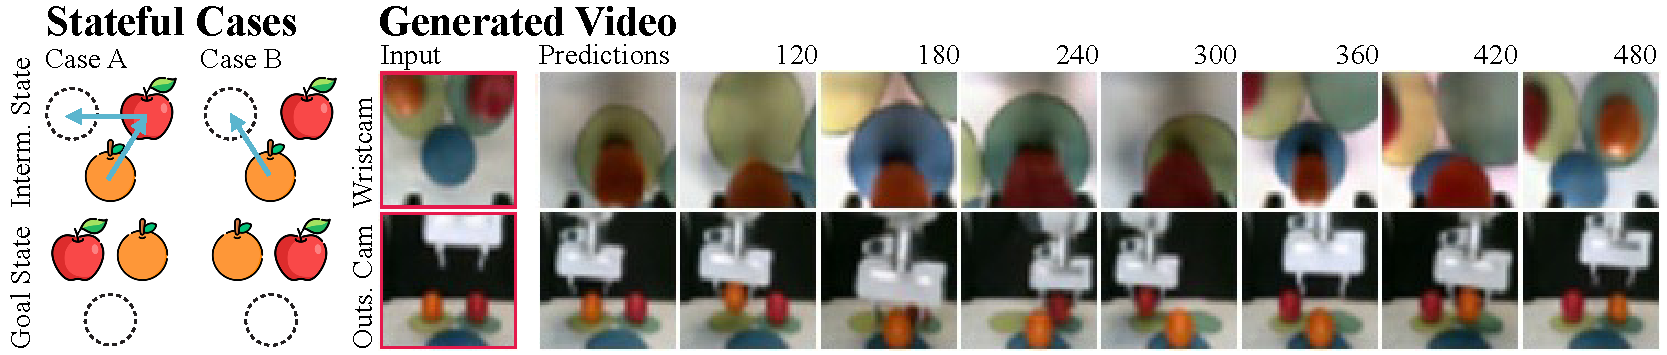
\includegraphics[width=\linewidth]{figures/pdf/Imitation.pdf}
    \caption{In our real robot task, a robot arm is asked to swap the slots of two fruits using a third slot. Since the fruits are input in random slots at the beginning, one cannot determine the next steps from a single observation without knowledge of the initial placement of the fruits. As illustrated in (a) and (b), the upper observation is the same but the desired outcome illustrated below can vary---the task thus requires remembering the initial configuration. In addition, as shown in (c), the same model that generates actions also synthesizes realistic video from just a single frame.}
    \label{fig:robot}
    \vspace{-10pt}
\end{figure*}

\subsection{Robotics: Long horizon imitation learning and robust visuomotor control}

\label{sec:exp_robot}
Finally, we illustrate that \algo{} (\algshort{}) opens up new opportunities in the visuomotor control of real-world robots. Imitation learning~\cite{chi2023diffusion} is a popular technique in robotic manipulation where one learns an observation-to-action mapping from expert demonstrations. However, the lack of memory often prevents imitation learning from accomplishing long-horizon tasks. \algshort{} not only alleviates this shortcoming but also provides a way to make imitation learning robust.

\paragraph{Imitation Learning with Memory.}
We collect a dataset of videos and actions by teleoperating with a Franka robot. In the chosen task, one needs to swap the position of an apple and an orange, using a third slot. See Fig.~\ref{fig:robot} for an illustration. The initial positions of the fruits are randomized such that there are two possible goal states. As illustrated in Fig.~\ref{fig:robot}, when one fruit is in the third slot, the desired outcome cannot be inferred from the current observation---a policy must remember the initial configuration to determine which fruit to move. In contrast to common behavior cloning methods, \algshort{} naturally incorporates memory in its latent state. We found that \algshort{} achieves $80\%$ success rate while diffusion policy~\cite{chi2023diffusion}, a state-of-the-art imitation learning algorithm without memory, fails. 

\paragraph{Robustness to missing or noisy observations.}
Because it incorporates principles from Bayes filtering, 
\algo{} can perform imitation learning while being robust to noisy or missing observations. We demonstrate this by adding visual distractions and even fully occluding the camera during execution.
\algshort{} allows us to easily indicate these observations as ``noisy'' by using $k>0$, in which case \algshort{} relies heavily on its prior model to predict actions. Consequently, the success rate is only lowered by $4\%$ to $76\%$.
In contrast, a next-frame diffusion model baseline attains a success rate of $48\%$: it must treat perturbed observations as ground truth and suffers out-of-distribution error. 

\paragraph{Potential for pre-training with video.} Finally, in parallel to generating actions, Fig.~\ref{fig:robot} illustrates that \algo{} is capable of generating a video of the robot performing the task given only an initial frame, unifying diffusion policy/imitation learning and video generative modeling and paving the way to pre-training on unlabeled video.

\subsection{Time Series Forecasting: \algo{} is a Good General-purpose Sequence Model}
In Appendix~\ref{app:exp_timeseries}, we show that \algshort{} is competitive with prior diffusion~\cite{rasul2021autoregressive} and transformer-based~\cite{rasul2021multivariate} work on multivariate time series forecasting, following the experimental setup of ~\cite{salinas2019highdimensional}. 


